\section{Basic User Interface Overview}
\subsection{Main Window Layout}
All user interaction takes place within the main window.  The main window is comprised of several movable widgets that can moved around or floating, depending on what best facilitates the work flow.  The main movable widgets are \ui{input}[input panel], \ui{properties panel},  \ui{3D view}, \ui{2D view}, and \ui{Mesh view}.  At start \ui{3D view}, \ui{2D view}, and \ui{Mesh view} are combined together in the visualization area, selectable by tab, but they can be moved.  There are two non-movable widgets.  The first non-movable widget is the \ui{toolbar}, located above the \ui{input}[input panel] and has icons for often used actions and the z-scaling controls.  The second non-movable widget is the \ui{menu}, located above the \ui{toolbar}. Refer to Figure \ref{fig:mainwindow1} to see these pictorally.

\begin{figure}[H]
	\begin{center}
		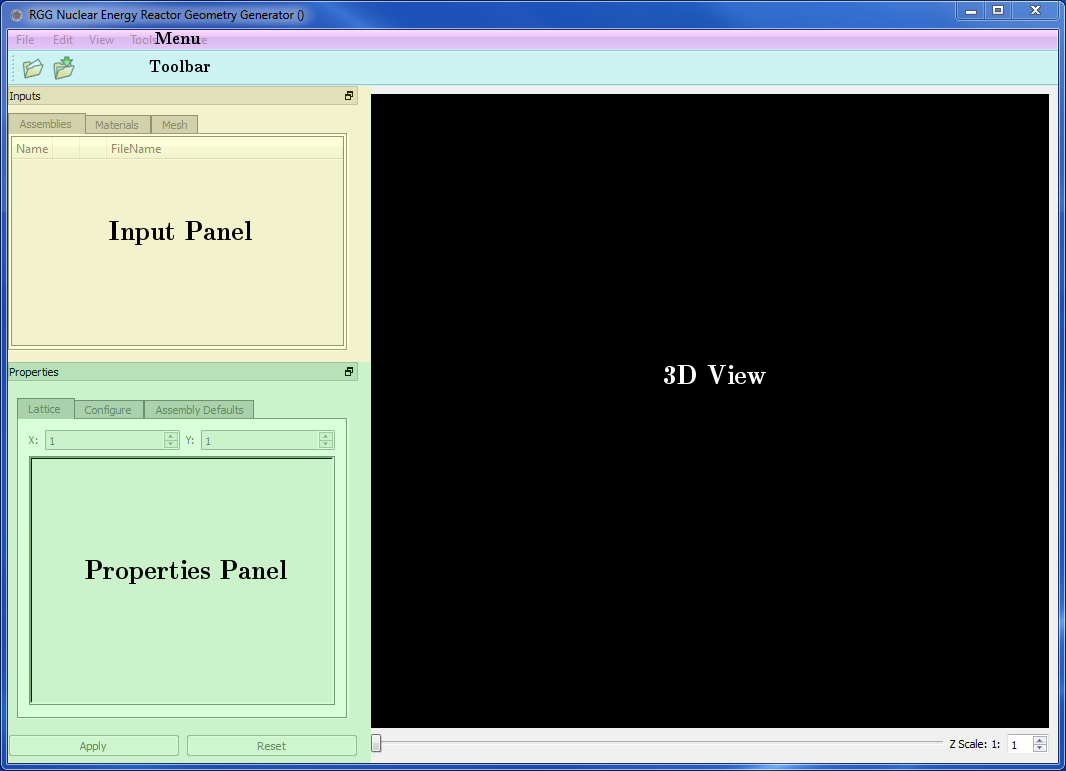
\includegraphics[width=\linewidth]{Images/main-window-layout.png}
		\caption{Layout of the \ui{main window}.}
		\label{fig:mainwindow1}
	\end{center}
\end{figure}


\subsection{Input Panel}
The \ui{input panel} has three tabs: the \ui{assemblies tab}, the \ui{materials tab}, and the \ui{mesh tab}.

\subsubsection{Assemblies Tab}
The \ui{assemblies tab} shows the hierarchal nature of the core, assemblies, pins and ducts.  Recall that a core is composed of assemblies which are placed in the core's lattice, and that these assemblies are in turn composed of pins and ducts that are placed in the assembly lattice.  When 

\begin{figure}[H]
	\begin{center}
		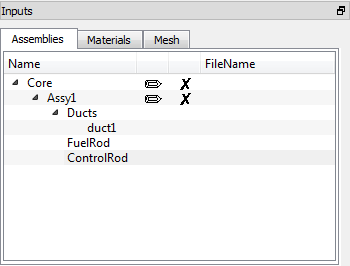
\includegraphics[width=0.5\linewidth]{Images/assemblies-tab.png}
		\caption{The assemblies tab shows the core, assembly, pin, and duct hierarchy.}
		\label{fig:mainwindow2}
	\end{center}
\end{figure}

Note you can check to see if the core or an assembly has had changes made to it since the last save.  A \ui{pencil icon} (as shown in Figure \ref{fig:mainwindow2}) indicates that edits have been made since the file was last saved.  A \ui{green box icon} indicates that the file is up to date.

You can also see the status of mesh files here.  An \ui{x icon} (as shown, to the right of the \ui{pencil icon}) indicates that mesh files have not been generated (or haven't been recreated since edits to the associated core or assembly), while \ui{green box icons} indicate that they are up to date.

\subsubsection{Materials Tab}
\toIndex{Materials}
The \ui{materials tab} (Figure ~\ref{fig:mainwindow3}) details the list of available materials, their associated colors, and whether or not they are viewable.  You can use this tab to create, remove, import, and export materials, as well as edit the labels and colors of materials and toggle whether or not they are shown in the \ui{3D view} or \ui{Mesh view}.  You can also filter the list based on materials used in the core or currently displayed in either the \ui{3D view} or \ui{Mesh view}.

\begin{figure}[h]
	\begin{center}
		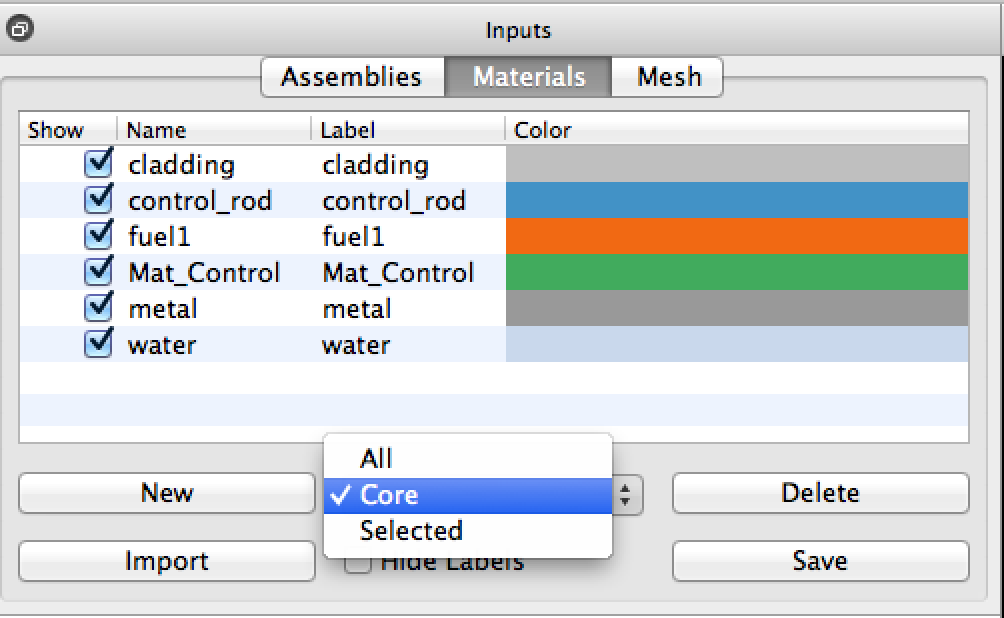
\includegraphics[width=0.5\linewidth]{Images/materials-tab.png}
		\caption{The materials tab shows available materials.}
		\label{fig:mainwindow3}
	\end{center}
\end{figure}

\subsubsection{Mesh Tab}
The \ui{mesh tab} (Figure ~\ref{fig:mainwindow4}) allows you to control the viewing of the mesh.  It is only available when a mesh is loaded.  It has the options to control what shows up in the \ui{Mesh view}, including the ability to show volumes, boundaries, surfaces, Neumann sets, Dirichlet sets, Material sets, show mesh edges, and to colorize the different volumes.  More information on this tab is given in Section \ref{section:DisplayingMeshes}.

\begin{figure}[h]
	\begin{center}
		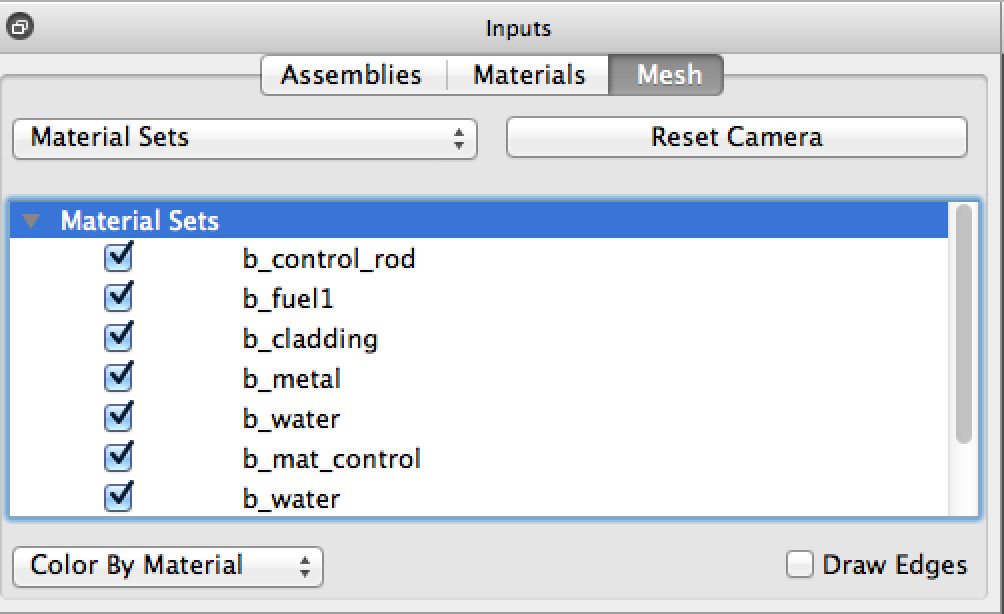
\includegraphics[width=0.5\linewidth]{Images/mash-tab.png}
		\caption{Used to control the mesh}
		\label{fig:mainwindow4}
	\end{center}
\end{figure}

\subsection{Properties Panel}
The \ui{properties panel} changes depending on the current state of the input panel's \ui{assemblies tab}.

\begin{itemize}
	\item{If you're clicking on a core, it will display three tabs: the \ui{lattice tab}, the \ui{configure tab}, and the \ui{assembly defaults tab}.}
	\item{If you're clicking on an assembly, it will display the \ui{lattice tab} and \ui{configure tab}.  Note that the assembly has a different \ui{lattice tab} and \ui{configure tab} from the core.}
	\item{If you're clicking on a duct, it will display the \ui{duct tab}.}
	\item{If you're clicking on a pin, it will display the \ui{pin tab}.}
\end{itemize}

\subsubsection{Lattice Tab}
The \ui{lattice tab} controls the number of layers (in a hexagonal core) or the dimensions (in a rectilinear core) to get the desired lattice geometry.  For cores, it also controls the \ui{Reactor Vessel} and \ui{Boundary Layer}s.  For assemblies, there is a checkbox to allow for auto-centering the pins.  Also for assemblies, this tab controls the \ui{2D view} color and label.  There is also controls for assembly rotation and the \ui{duct} used.  See Figure \ref{fig:latticetab}.

\begin{figure}
\centering
\begin{subfigure}{.5\textwidth}
  \centering
  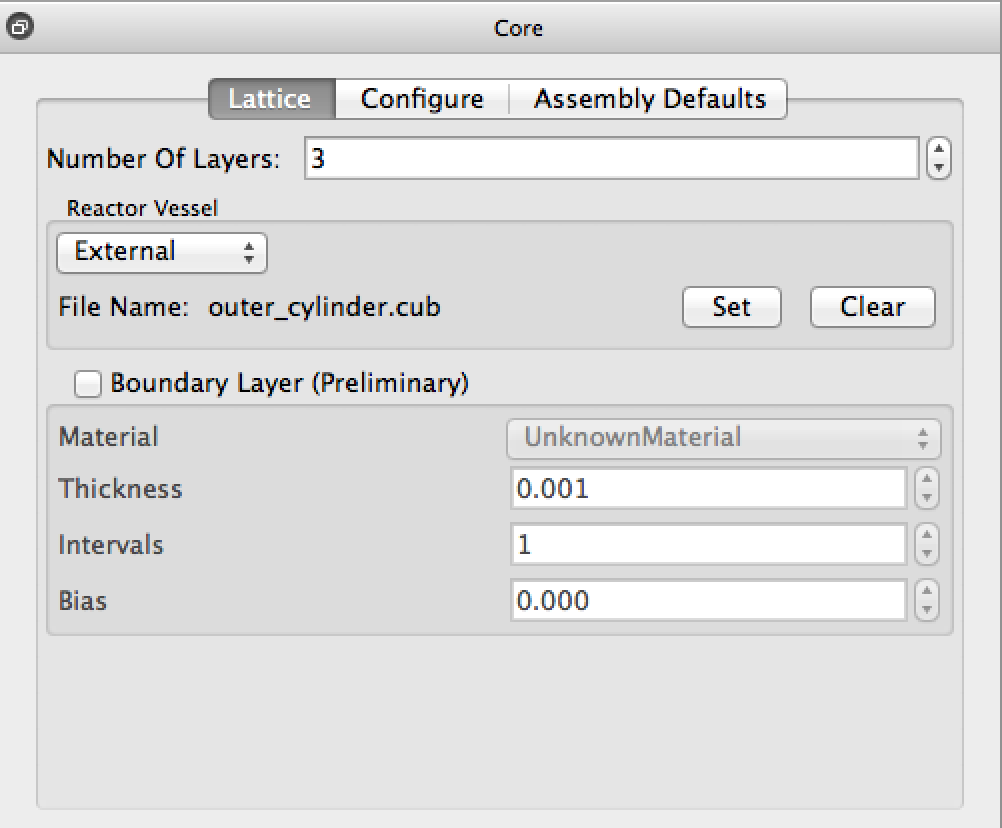
\includegraphics[width=0.6\linewidth]{Images/core-lattice.png}
  \caption{Core Lattice Tab.}
  \label{fig:rectSetMaterial}
\end{subfigure}%
\begin{subfigure}{.5\textwidth}
  \centering
  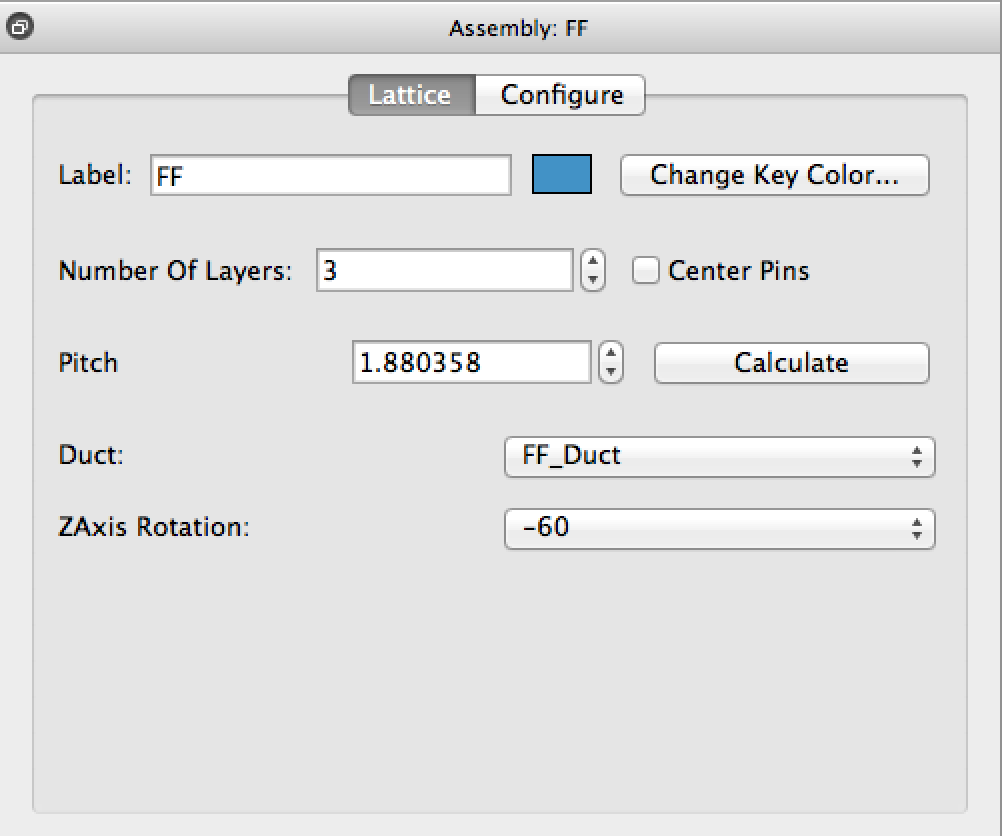
\includegraphics[width=0.6\linewidth]{Images/assy-lattice.png}
  \caption{The Assembly Lattice Tab.}
  \label{fig:rectDuctResult}
\end{subfigure}
\caption{The two versions of the Lattice Tab.}
\label{fig:latticetab}
\end{figure}


\subsubsection{Configure Tab}
This tab allows you to customize other meshing parameters from MeshKit files which are not currently provided an interface in the GUI. See Chapter \ref{chapter:Meshing} for information on how to mesh your core.

\subsubsection{Assembly Defaults Tab}
The \ui{assembly defaults tab} allows you to specify general meshing information.  You can set whether the mesh you want to generate will be tetrahedral or hexahedral, and also change the default dimensions of the ducts comprising your core.  Changing these values will propagate all the way down to every component, so you can change it all in one place instead of adjusting the height of every duct in every assembly.

\subsubsection{Duct Tab}
The \ui{duct tab} exposes the different configuration options for a duct piece.  You can change the position and dimensional settings towards the top, the duct pitch, and the duct material (with associated normalized thickness, if desired).

\subsubsection{Pin Tab}
The \ui{pin tab} allows you to change the key color of the pin, specify the pin material(s), and create, remove, or edit pin pieces.

\subsection{3D View}
The \ui{3D view} (Figure ~\ref{fig:3DView}) displays a representation of the current component.  You can use the following controls to interact with it:

\begin{itemize}
	\item{To rotate, click with the left mouse button.}
	\item{To pan, either shift-click with the left mouse button or use the middle mouse button.}
	\item{To zoom, click with the right mouse button.}
\end{itemize}

\begin{figure}[h]
	\begin{center}
		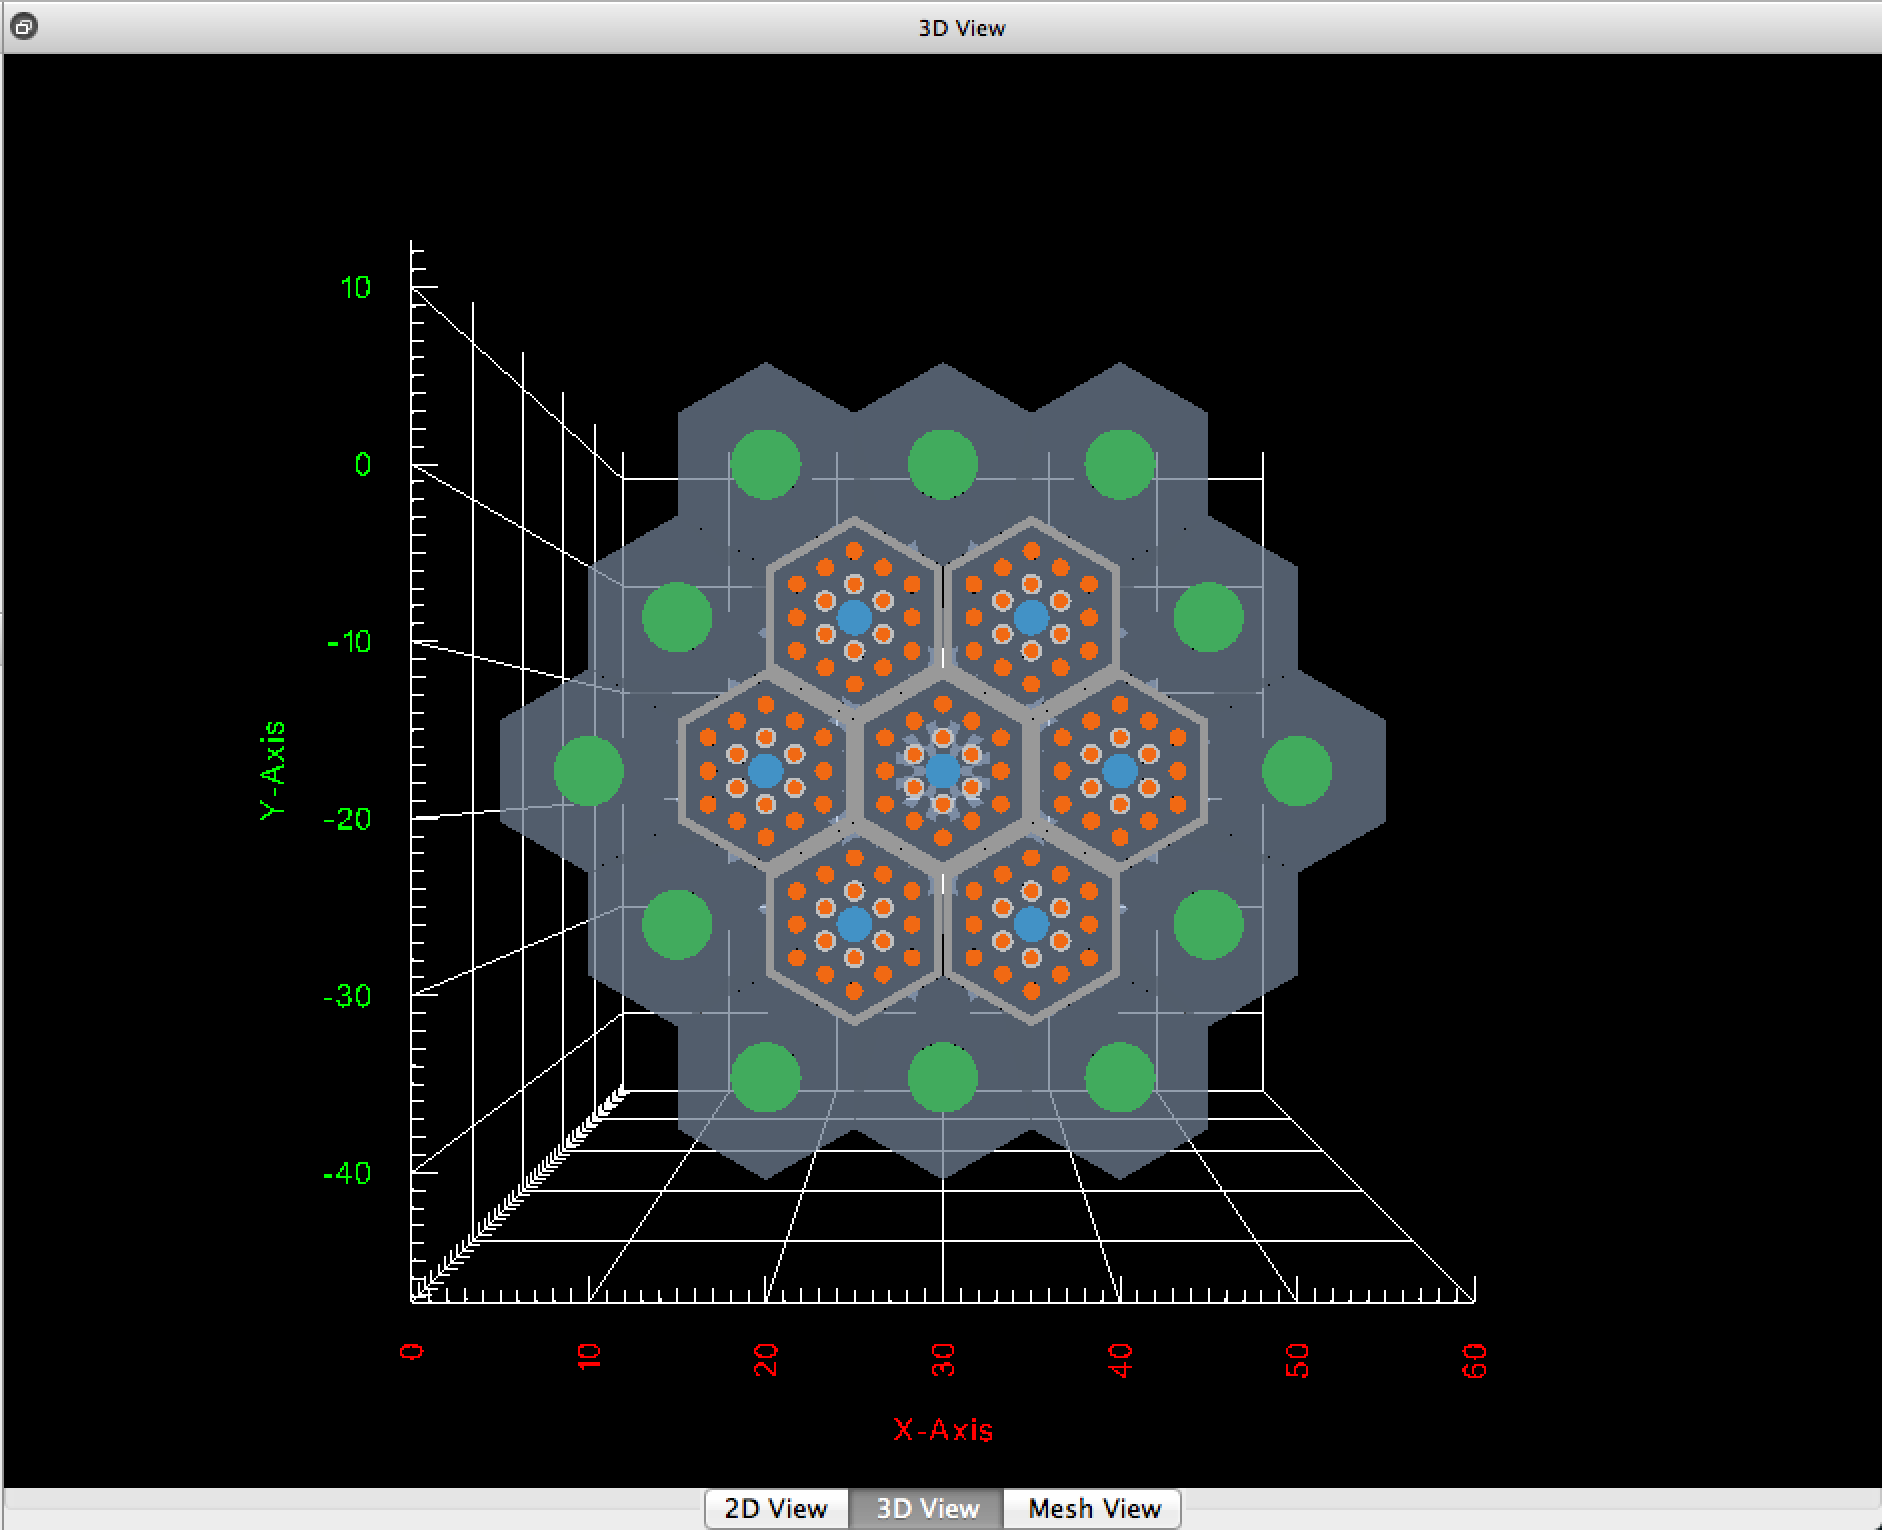
\includegraphics[width=0.5\linewidth]{Images/3DView.png}
		\caption{The 3D View}
		\label{fig:3DView}
	\end{center}
\end{figure}

Similar to the \ui{properties panel}, the \ui{3D view} changes depending on what is selected in the assemblies tab of the input panel.

\begin{itemize}
	\item{If you're clicking on a core, it will display the entire core.}
	\item{If you're clicking on an assembly or a duct, it will display the assembly.}
	\item{If you're clicking on a pin, it will display the pin.}
\end{itemize}

\subsection{2D View}
The \ui{2D view} (Figure ~\ref{fig:2DView}) provides a 2d schematic of the core or assembly depending which is selected. Each assembly or pin represented here will be filled with its corresponding key color.

You can edit this information by moving you mouse over the cell you want to edit and then right-click on each cell to select the desired assembly or pin.  In the pop-up menu, there are options to \ui{Replace All With} and \ui{Fill Ring With}. \ui{Replace All With} replaces every cell that is same component with the desired assembly or pin.  \ui{Fill Ring With} fills every cell in the ring with the desired assembly or pin.  Alternatively, you can drag and drop an existing component onto the cell.

\begin{figure}[h]
	\begin{center}
		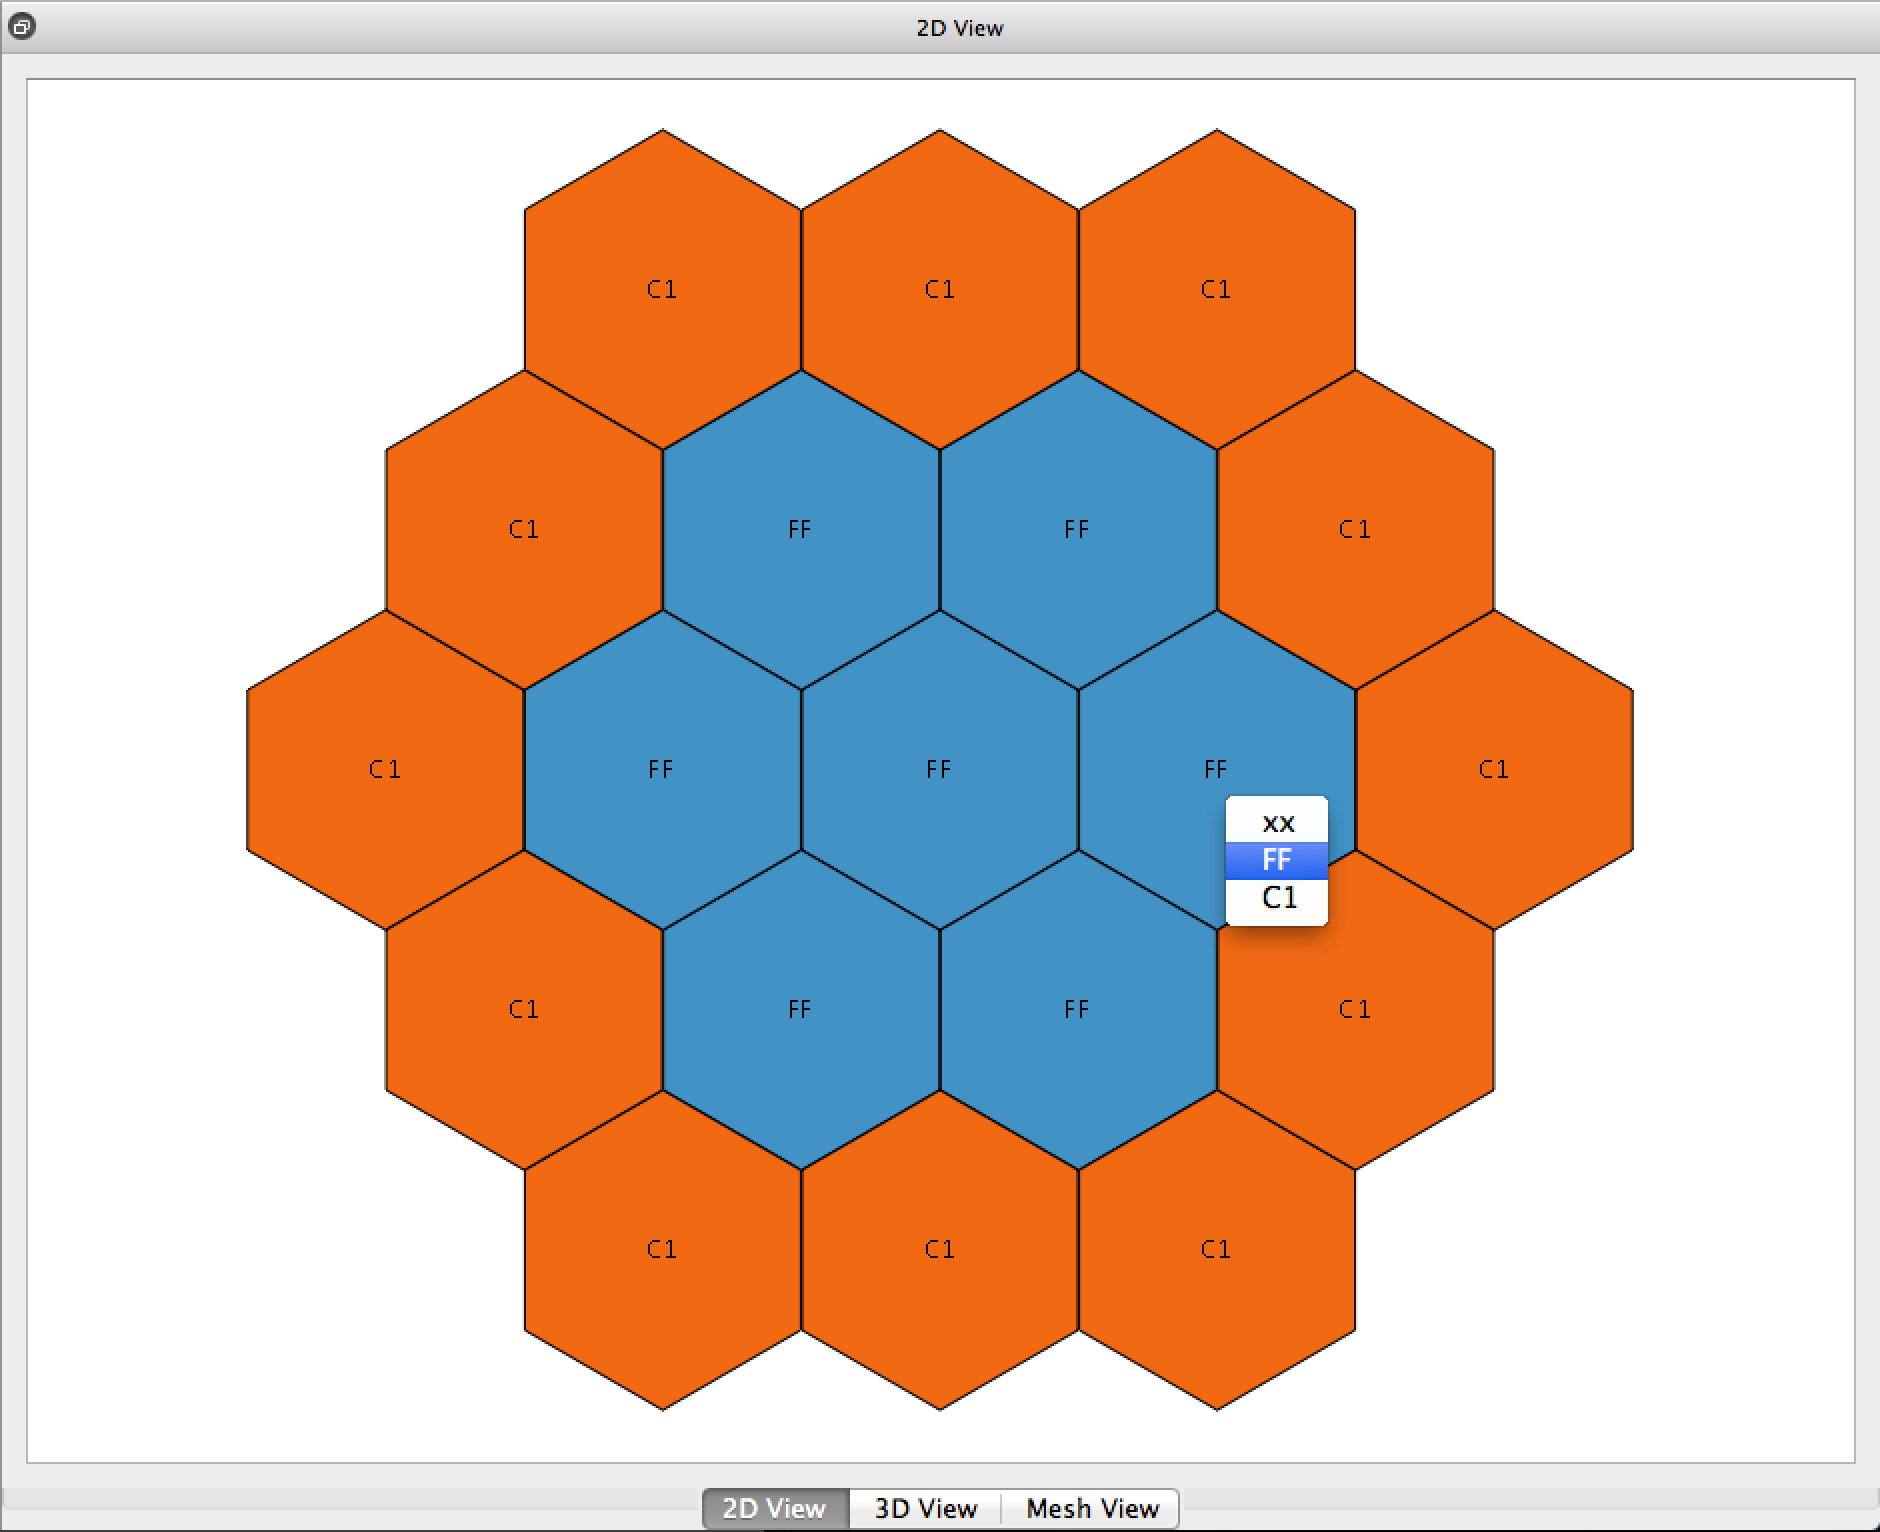
\includegraphics[width=0.5\linewidth]{Images/2DView.png}
		\caption{The 2D View}
		\label{fig:2DView}
	\end{center}
\end{figure}

\subsection{Mesh View}
The \ui{Mesh view} (Figure ~\ref{fig:MeshView}) is only visible if a mesh has been loaded.  The Mesh Tab controls what is displayed here.

\begin{figure}[h]
	\begin{center}
		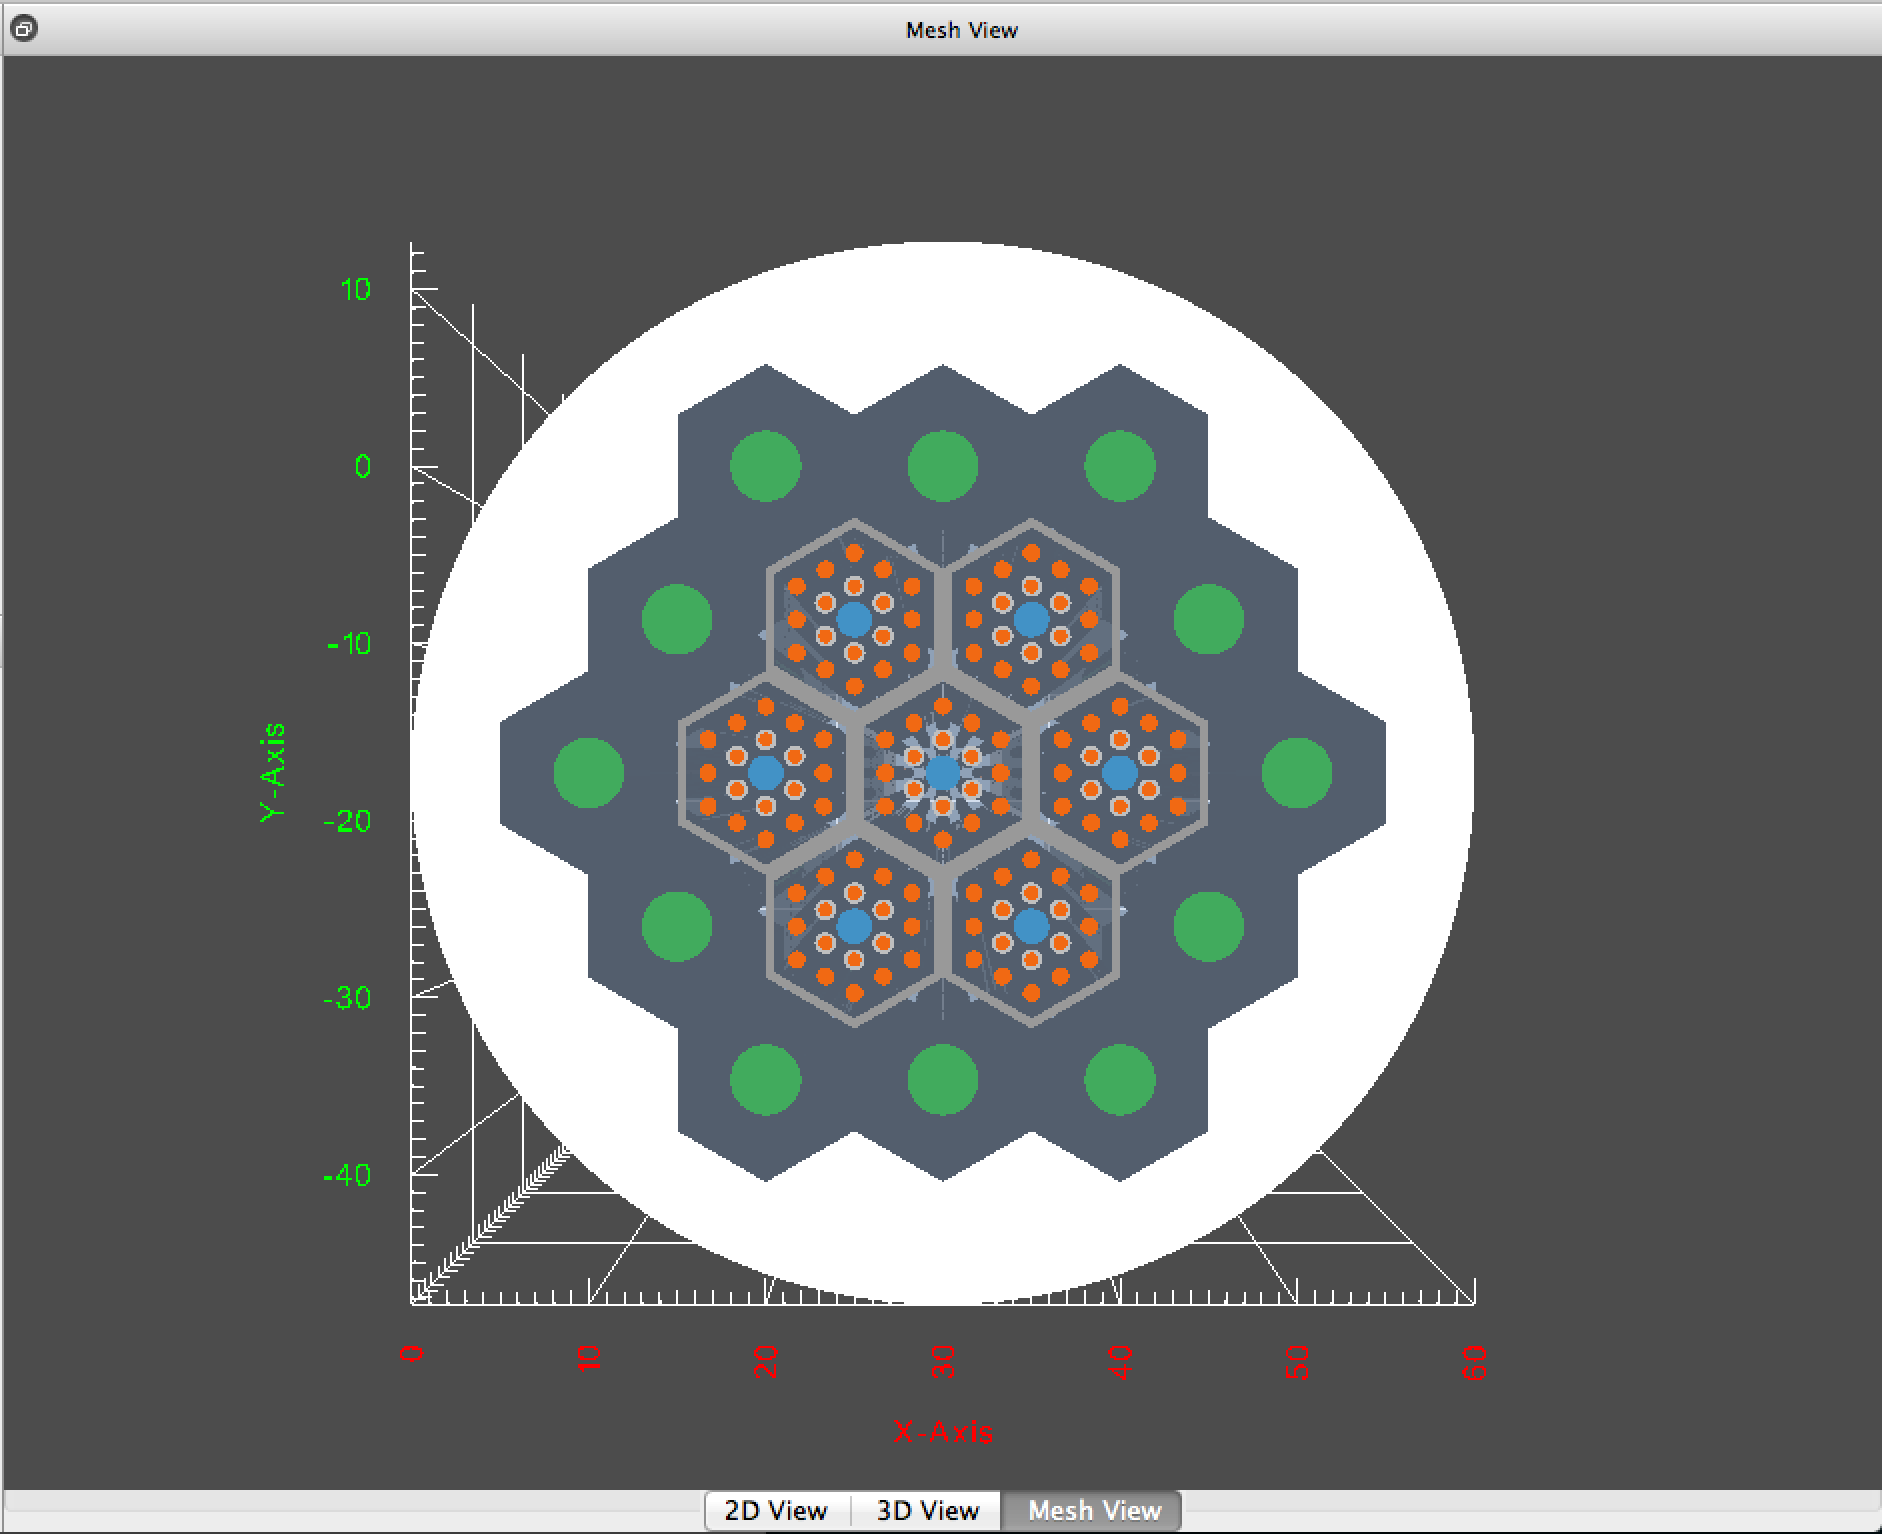
\includegraphics[width=0.5\linewidth]{Images/MeshView.png}
		\caption{The Mesh View}
		\label{fig:MeshView}
	\end{center}
\end{figure}

